% Options for packages loaded elsewhere
\PassOptionsToPackage{unicode}{hyperref}
\PassOptionsToPackage{hyphens}{url}
%
\documentclass[
  ignorenonframetext,
  brazilian,
]{beamer}
\usepackage{pgfpages}
\setbeamertemplate{caption}[numbered]
\setbeamertemplate{caption label separator}{: }
\setbeamercolor{caption name}{fg=normal text.fg}
\beamertemplatenavigationsymbolsempty
% Prevent slide breaks in the middle of a paragraph
\widowpenalties 1 10000
\raggedbottom
\setbeamertemplate{part page}{
  \centering
  \begin{beamercolorbox}[sep=16pt,center]{part title}
    \usebeamerfont{part title}\insertpart\par
  \end{beamercolorbox}
}
\setbeamertemplate{section page}{
  \centering
  \begin{beamercolorbox}[sep=12pt,center]{section title}
    \usebeamerfont{section title}\insertsection\par
  \end{beamercolorbox}
}
\setbeamertemplate{subsection page}{
  \centering
  \begin{beamercolorbox}[sep=8pt,center]{subsection title}
    \usebeamerfont{subsection title}\insertsubsection\par
  \end{beamercolorbox}
}
\AtBeginPart{
  \frame{\partpage}
}
\AtBeginSection{
  \ifbibliography
  \else
    \frame{\sectionpage}
  \fi
}
\AtBeginSubsection{
  \frame{\subsectionpage}
}

\usepackage{amsmath,amssymb}
\usepackage{iftex}
\ifPDFTeX
  \usepackage[T1]{fontenc}
  \usepackage[utf8]{inputenc}
  \usepackage{textcomp} % provide euro and other symbols
\else % if luatex or xetex
  \usepackage{unicode-math}
  \defaultfontfeatures{Scale=MatchLowercase}
  \defaultfontfeatures[\rmfamily]{Ligatures=TeX,Scale=1}
\fi
\usepackage{lmodern}
\usetheme[]{Berlin}
\ifPDFTeX\else  
    % xetex/luatex font selection
\fi
% Use upquote if available, for straight quotes in verbatim environments
\IfFileExists{upquote.sty}{\usepackage{upquote}}{}
\IfFileExists{microtype.sty}{% use microtype if available
  \usepackage[]{microtype}
  \UseMicrotypeSet[protrusion]{basicmath} % disable protrusion for tt fonts
}{}
\makeatletter
\@ifundefined{KOMAClassName}{% if non-KOMA class
  \IfFileExists{parskip.sty}{%
    \usepackage{parskip}
  }{% else
    \setlength{\parindent}{0pt}
    \setlength{\parskip}{6pt plus 2pt minus 1pt}}
}{% if KOMA class
  \KOMAoptions{parskip=half}}
\makeatother
\usepackage{xcolor}
\newif\ifbibliography
\setlength{\emergencystretch}{3em} % prevent overfull lines
\setcounter{secnumdepth}{-\maxdimen} % remove section numbering


\providecommand{\tightlist}{%
  \setlength{\itemsep}{0pt}\setlength{\parskip}{0pt}}\usepackage{longtable,booktabs,array}
\usepackage{calc} % for calculating minipage widths
\usepackage{caption}
% Make caption package work with longtable
\makeatletter
\def\fnum@table{\tablename~\thetable}
\makeatother
\usepackage{graphicx}
\makeatletter
\newsavebox\pandoc@box
\newcommand*\pandocbounded[1]{% scales image to fit in text height/width
  \sbox\pandoc@box{#1}%
  \Gscale@div\@tempa{\textheight}{\dimexpr\ht\pandoc@box+\dp\pandoc@box\relax}%
  \Gscale@div\@tempb{\linewidth}{\wd\pandoc@box}%
  \ifdim\@tempb\p@<\@tempa\p@\let\@tempa\@tempb\fi% select the smaller of both
  \ifdim\@tempa\p@<\p@\scalebox{\@tempa}{\usebox\pandoc@box}%
  \else\usebox{\pandoc@box}%
  \fi%
}
% Set default figure placement to htbp
\def\fps@figure{htbp}
\makeatother

\input{../main/configs/rspalette.tex}

\usepackage{amsmath}
\usepackage{mathtools}
\usepackage{float}
\usepackage{multirow}
\usepackage{multicol}

\usepackage{tikz}
\usetikzlibrary{positioning}
\usetikzlibrary{decorations.pathreplacing}
\usepackage{algorithm}
\usepackage{algpseudocode}

%\usepackage{caption}
\captionsetup[table]{name=Tabela}
\captionsetup[figure]{name=Figura}
\captionsetup[table]{skip=0pt, belowskip=0pt}
\captionsetup[figure]{skip=0pt, belowskip=0pt}
\setlength{\belowcaptionskip}{1pt plus 1pt minus 3pt}

\newcommand{\sgp}{\text{sgp}}
\newcommand{\rgp}{\text{rgp}}
\newcommand{\dgp}{\text{dgp}}
\renewcommand{\mod}{\text{mod}}

\setbeamertemplate{footline}{}
\makeatletter
\@ifpackageloaded{caption}{}{\usepackage{caption}}
\AtBeginDocument{%
\ifdefined\contentsname
  \renewcommand*\contentsname{Índice}
\else
  \newcommand\contentsname{Índice}
\fi
\ifdefined\listfigurename
  \renewcommand*\listfigurename{Lista de Figuras}
\else
  \newcommand\listfigurename{Lista de Figuras}
\fi
\ifdefined\listtablename
  \renewcommand*\listtablename{Lista de Tabelas}
\else
  \newcommand\listtablename{Lista de Tabelas}
\fi
\ifdefined\figurename
  \renewcommand*\figurename{Figura}
\else
  \newcommand\figurename{Figura}
\fi
\ifdefined\tablename
  \renewcommand*\tablename{Tabela}
\else
  \newcommand\tablename{Tabela}
\fi
}
\@ifpackageloaded{float}{}{\usepackage{float}}
\floatstyle{ruled}
\@ifundefined{c@chapter}{\newfloat{codelisting}{h}{lop}}{\newfloat{codelisting}{h}{lop}[chapter]}
\floatname{codelisting}{Listagem}
\newcommand*\listoflistings{\listof{codelisting}{Lista de Listagens}}
\makeatother
\makeatletter
\makeatother
\makeatletter
\@ifpackageloaded{caption}{}{\usepackage{caption}}
\@ifpackageloaded{subcaption}{}{\usepackage{subcaption}}
\makeatother

\ifLuaTeX
\usepackage[bidi=basic]{babel}
\else
\usepackage[bidi=default]{babel}
\fi
\babelprovide[main,import]{brazilian}
% get rid of language-specific shorthands (see #6817):
\let\LanguageShortHands\languageshorthands
\def\languageshorthands#1{}
\usepackage{bookmark}

\IfFileExists{xurl.sty}{\usepackage{xurl}}{} % add URL line breaks if available
\urlstyle{same} % disable monospaced font for URLs
\hypersetup{
  pdftitle={Semião 2026 - Apresentação},
  pdfauthor={Ricardo Semião e Castro},
  pdflang={pt-BR},
  pdfsubject={Master's Thesis in Economics at FGV-EESP},
  pdfkeywords={Time series, Regime Switching},
  hidelinks,
  pdfcreator={LaTeX via pandoc}}


\title{Regimes' Characteristics and Time Series Forecasting}
\subtitle{FGV-EESP Masters' Thesis}
\author{Ricardo Semião e Castro\\
Orientador: Marcelo Fernandes}
\date{20 mai 2026}

\begin{document}
\frame{\titlepage}


\section{Introdução}\label{introduuxe7uxe3o}

\begin{frame}{Objetivo}
\phantomsection\label{objetivo}
\textbf{Pergunta de pesquisa:}

\begin{itemize}
\tightlist
\item
  Como modelos de mudança de regimes (RS) desempenham em diferentes
  processos geradores de dados (DGPs)?
\item
  Como esse desempenho se relaciona com características das
  distribuições dos regimes?
\end{itemize}

\pause

Mudança de regime: comportamento alterna entre dois ou mais padrões; DGP
alterna entre conjuntos de parâmetros.

\pause

Comportamento observável nos dados, e útil para modelar
não-linearidades, outliers, entre outros.
\end{frame}

\begin{frame}{Exemplos de mudanças de regime}
\phantomsection\label{exemplos-de-mudanuxe7as-de-regime}
\begin{figure}

\caption{\label{fig-selic_reservas}Regimes monetários do BC}

\centering{

\includegraphics[width=\linewidth,height=0.6\textheight,keepaspectratio]{../../personal/tests/selic_reservas.png}

}

\end{figure}%

\small Fonte: Lima et al.~(2007) ``Monetary policy regimes in Brazil''
(\href{http://repositorio.ipea.gov.br/handle/11058/1884}{link}).
\normalsize
\end{frame}

\begin{frame}{Exemplos de mudanças de regime}
\phantomsection\label{exemplos-de-mudanuxe7as-de-regime-1}
\begin{figure}

\caption{\label{fig-ws_forecast}Vento no noroeste dos EUA}

\centering{

\includegraphics[width=\linewidth,height=0.6\textheight,keepaspectratio]{../../personal/tests/ws_forecast.png}

}

\end{figure}%

\small Fonte: Gneiting et al.~(2012) ``Calibrated Probabilistic
Forecasting at the Stateline Wind Energy Center''
(\href{https://doi.org/10.1198/016214506000000456}{link}). \normalsize
\end{frame}

\begin{frame}{Características dos regimes}
\phantomsection\label{caracteruxedsticas-dos-regimes}
Estudar o desempenho desses modelos é importante, e as características
(métricas) dos regimes são relevantes.

\pause

\vspace{0.5cm}

\begin{figure}

\caption{\label{fig-ws_boxplots}Vento no noroeste dos EUA -
Distribuições}

\centering{

\includegraphics[width=\linewidth,height=0.4\textheight,keepaspectratio]{../../personal/tests/ws_boxplots.png}

}

\end{figure}%

\small Fonte: Gneiting et al.~(2012). \normalsize
\end{frame}

\begin{frame}{Resumo da metodologia}
\phantomsection\label{resumo-da-metodologia}
\begin{enumerate}
\item
  Definir uma estrutura geral dos DGPs, modelos, e métricas dos regimes.
\item
  Gerar séries, previsões, e métricas via simulação de Monte Carlo.
\item
  Estudar os DGPs e performance dos modelos.
\end{enumerate}
\end{frame}

\begin{frame}{Literatura relacionada}
\phantomsection\label{literatura-relacionada}
Literaturas similares:

\begin{itemize}
\tightlist
\item
  Modelos de estado-espaço.
\item
  Modelos de quebras estruturais.
\end{itemize}

\pause

Literatura de RS:

\begin{itemize}
\tightlist
\item
  Quebras abruptas vs.~suaves.
\item
  Processos determinísticos vs.~estocásticos.
\item
  \emph{Markov Switching} (MS), \emph{Self-Exciting Threshold} (SET),
  \emph{Smooth Transition} (ST).
\item
  Modelos `agnósticos': K-means (KM), Random Forest (RF), Neural
  Network.
\end{itemize}
\end{frame}

\section{Metodologia}\label{metodologia}

\begin{frame}{Processos de mudança de regime}
\phantomsection\label{processos-de-mudanuxe7a-de-regime}
\begin{figure}[H]

\caption{\label{fig-tik}A estrutura de um processo de RS}

\centering{

\begin{tikzpicture}[font=\sffamily]
% Styles:
\tikzset{mybrace/.style={decorate, decoration={brace, amplitude=10pt, raise=1.3ex}}}
\tikzset{node distance = 0.25cm and 0.1cm}

% Main nodes:
\node[] (dgp) {DGP};
\node[] (e)   [right = 0.25cm of dgp] {$=$};
\node[] (sgp) [right = 0.25cm of e] {SGP};
\node[] (p)   [right = 1.95cm of sgp] {\&};
\node[] (rgp) [right = 1.95cm of p] {RGP};

% Lower nodes:
\node[] (p2)   [below = 0.5cm of sgp] {\&};
\node[] (csgp) [left  = of p2] {functional form};
\node[] (rsch) [right = of p2] {regime nature};

% Math:
\node[] (msgp)  [above = of sgp] {$y_t = \sgp(y_{1:(t-1)}, r_{1:t} ~;~ \Theta_y^s) \cdot r_t^s$};
\node[] (mrgp)  [above = of rgp] {$r_t = \rgp(y_{1:(t-1)}, r_{1:(t-1)} ~;~ \Theta_r)$};
\node[] (mcsgp) [below = 0.35cm of csgp] {$f_{\sgp}$};
\node[] (mrsch) [below = of rsch] {$\{\Theta^1_y, \dots, \Theta^s_y\}$};

% Braces using the defined style, add mirror in place:
\draw[mybrace]         (csgp.west) -- (rsch.east);
\draw[mybrace, decoration={mirror}] (mrgp.west) -- (mrgp.east);
\draw[mybrace, decoration={mirror}] (msgp.west) -- (msgp.east);
\draw[mybrace, decoration={amplitude=8pt}]         (mcsgp.west) -- (mcsgp.east);
\draw[mybrace]         (mrsch.west) -- (mrsch.east);
\end{tikzpicture}

}

\end{figure}%

\pause

Exemplos:

\begin{itemize}
\tightlist
\item
  RGP: regime 1 se a série passada foi alta, 2 c.c.
\item
  SGP: \(AR(1)\) com interceptos diferentes em cada regime.
\end{itemize}
\end{frame}

\begin{frame}{SGPs consideradas}
\phantomsection\label{sgps-consideradas}
\textbf{Forma funcional:} \(AR(1)\), estacionário, com erros Gaussianos.

\pause

\textbf{Naturezas dos regimes:}

\begin{itemize}
\tightlist
\item
  Mudança em \(\mu\): (\(\mu^1 = 0\), \(\mu^2 = 0.5\)) e (\(\mu^1 = 0\),
  \(\mu^2 = 1\)).
\item
  Mudança em \(\rho\): (\(\rho_1^1 = 0.4\), \(\rho_1^2 = 0.6\)) e
  (\(\rho_1^1 = 0.2\), \(\rho_1^2 = 0.8\)).
\item
  Mudança em \(\sigma\): (\(\sigma^1 = 1\), \(\sigma^2 = 1.5\)) e
  (\(\sigma^1 = 1\), \(\sigma^2 = 2\)).
\end{itemize}
\end{frame}

\begin{frame}{RGPs e modelos considerados}
\phantomsection\label{rgps-e-modelos-considerados}
\textbf{RGPs:}

\begin{itemize}
\tightlist
\item
  Sem RS: sempre no regime 1.
\item
  SET e ST: baseados em \(y_{t-1}\).
\item
  MS: distribuição geométrica.
\item
  Todos com \(S = 2\) regimes, uma versão simétrica (\(\approx\) 50-50),
  e outra assimétrica (\(\approx\) 75-25).
\end{itemize}

\pause

\textbf{Modelos:}

\begin{itemize}
\tightlist
\item
  Recebem \(y\), geram parâmetros, \(\hat{r}\) e \(\hat{y}\).
\item
  MS, SET, e ST.
\item
  K-means e Random Forest, com 4 lags de \(y\), média, desvio-padrão, e
  \(ACF(1)\) móveis.
\item
  Todos os parâmetros mudam; assume-se 2 regimes.
\end{itemize}
\end{frame}

\begin{frame}{Métricas dos regimes}
\phantomsection\label{muxe9tricas-dos-regimes}
Métrica condicional nos regimes: \((y, r) \mapsto \mathbb{R}^{S}\).

Diferença entre os regimes:
\((y, r) \mapsto \mathbb{R}^{S} \mapsto \mathbb{R}\).

\pause

\textbf{Métricas:}

\begin{itemize}
\tightlist
\item
  Média, desvio-padrão, e \(ACF(1)\).
\item
  Outras métricas: RMSE, \(R^{2}\), e ajuste do regime.
\end{itemize}

\pause

Questões técnicas:

\begin{itemize}
\tightlist
\item
  Calculadas analiticamente, via \((y, r)\), ou \((y, \hat{r})\).
\item
  Podem requerer estacionariedade dentro de cada regime.
\end{itemize}
\end{frame}

\begin{frame}{Simulação de Monte Carlo}
\phantomsection\label{simulauxe7uxe3o-de-monte-carlo}
Estrutura:

\begin{itemize}
\tightlist
\item
  Para cada DGP e simulação:

  \begin{itemize}
  \tightlist
  \item
    Gerar erros aleatórios.
  \item
    Gerar \((y, r)\) via \(r_1 \to y_1 \to r_2 \to y_2 \to \dots\).
  \item
    Para cada modelo:

    \begin{itemize}
    \tightlist
    \item
      Obter \(\hat{y}\) e \(\hat{r}\).
    \item
      Calcular as métricas, gerando um dataset.
    \end{itemize}
  \end{itemize}
\end{itemize}

\pause

Hiperparâmetros:

\begin{itemize}
\tightlist
\item
  6 RNs, 7 RGPs e 5 modelos.
\item
  Número de simulações: 500.
\item
  Tamanho da série: 100, +4 descartes e +10 previsões.
\item
  Previsões com janela fixa:
  \(E_{1:T}[y_{T+h} \mid y_{1:(T + h - 1)}]\).
\end{itemize}

Implementação em R
(\href{https://github.com/ricardo-semiao/article-regime-id-performance}{link}),
paralelizado, reproduzível e expansível.
\end{frame}

\begin{frame}{Diagnósticos}
\phantomsection\label{diagnuxf3sticos}
\begin{table}[!htbp]

\caption{\label{tbl-estimation_issues}Problemas de estimação}

\centering{

\vspace{-0.4cm}
\resizebox{\textwidth}{!}{%
    \begin{tabular}{@{\extracolsep{\fill}}l|rrrr}
\toprule
 & Bad obs. & \% Bad & \% Removed & Obs. left \\ 
\midrule\addlinespace[2.5pt]
Full sample & 0 & 0\% & 0\% & 126,000 \\ 
Bad convergence & 148 & 0.1\% & 0.1\% & 125,852 \\ 
NAs in parameters & 245 & 0.2\% & 0.2\% & 125,607 \\ 
Low \#obs. in regimes & 967 & 0.8\% & 0.6\% & 124,859 \\ 
Unreasonable parameters & 1,803 & 1.4\% & 1.3\% & 123,162 \\ 
Unreasonable errors & 145 & 0.1\% & 0\% & 123,137 \\ 
{\bfseries Total} & {\bfseries 3,308} & {\bfseries 2.6\%} & {\bfseries 2.3\%} & {\bfseries 123,137} \\ 
\bottomrule
\end{tabular}
%
}

}

\end{table}%

Outros: aleatoriedade dos erros; comparação `verdadeiro vs.~estimado' de
parâmetros e métricas; independência do índice de simulação.
\end{frame}

\section{Distribuições dos
regimes}\label{distribuiuxe7uxf5es-dos-regimes}

\begin{frame}{Diferenças entre os regimes}
\phantomsection\label{diferenuxe7as-entre-os-regimes}
\begin{table}[!htbp]

\caption{\label{tbl-metrics_sep_t}Separação dos regimes em cada DGP}

\centering{

\resizebox{\textwidth}{!}{%
    \begin{table}[t]
\fontsize{12.0pt}{14.0pt}\selectfont
\begin{tabular*}{\linewidth}{@{\extracolsep{\fill}}l|l|cccccc}
\toprule
\multicolumn{2}{l}{} & \multicolumn{2}{c}{{\(d(\hat{\mu}(.))\)}} & \multicolumn{2}{c}{{\(d(\hat{\rho}_1(.))\)}} & \multicolumn{2}{c}{{\(d(\hat{\sigma}(.))\)}} \\ 
\cmidrule(lr){3-4} \cmidrule(lr){5-6} \cmidrule(lr){7-8}
RGP & Param. \textbackslash{} RN & \((0, 0.5)\) & \((0, 1)\) & \((0.1, 0.9)\) & \((0.4, 0.6)\) & \((1, 1.5)\) & \((1, 2)\) \\ 
\midrule\addlinespace[2.5pt]
MS & \(\mu\) & .74 (.01)*** & 1.54 (.05)*** & .01 (0) & .02 (.05) & .04 (0) & .07 (.01) \\ 
 & \(\rho_{1}\) & .04 (.05) & .13 (.26) & .17 (.05)*** & .31 (.04)*** & .11 (0)** & .45 (.14)*** \\ 
 & \(\sigma\) & .1 (.11) & .11 (.27) & .03 (.03) & .01 (.03) & .55 (.01)*** & 1.08 (.12)*** \\ 
SET & \(\mu\) & 1.55 (.11)*** & 2.22 (.23)*** & .03 (.01) & .2 (.04)*** & .03 (.06) & 0 (.11) \\ 
 & \(\rho_{1}\) & .94 (.05)*** & 1.29 (.23)*** & .01 (.01) & .17 (.05)*** & .02 (.07) & .17 (.1)*** \\ 
 & \(\sigma\) & 1.13 (.16)*** & 1.12 (.26)*** & .11 (.06)*** & .11 (.09)** & .48 (.09)*** & 1 (.11)*** \\ 
ST & \(\mu\) & .62 (.04)*** & .39 (.02)*** & .03 (.04) & .12 (.01)*** & .04 (.01) & .01 (0) \\ 
 & \(\rho_{1}\) & .88 (.03)*** & 1.12 (.07)*** & .22 (.04)*** & .43 (.02)*** & .15 (.03)*** & .26 (.01)*** \\ 
 & \(\sigma\) & 1.18 (.1)*** & 1.38 (.06)*** & .13 (.06)*** & .02 (0) & .29 (.01)*** & .49 (.12)*** \\ 
\bottomrule
\end{tabular*}
\end{table}

%
}

}

\end{table}%
\end{frame}

\begin{frame}{Separação estimada}
\phantomsection\label{separauxe7uxe3o-estimada}
\begin{figure}[!htbp]

\caption{\label{fig-metrics_diff}Diferença verdadeira vs.~estimada}

\centering{

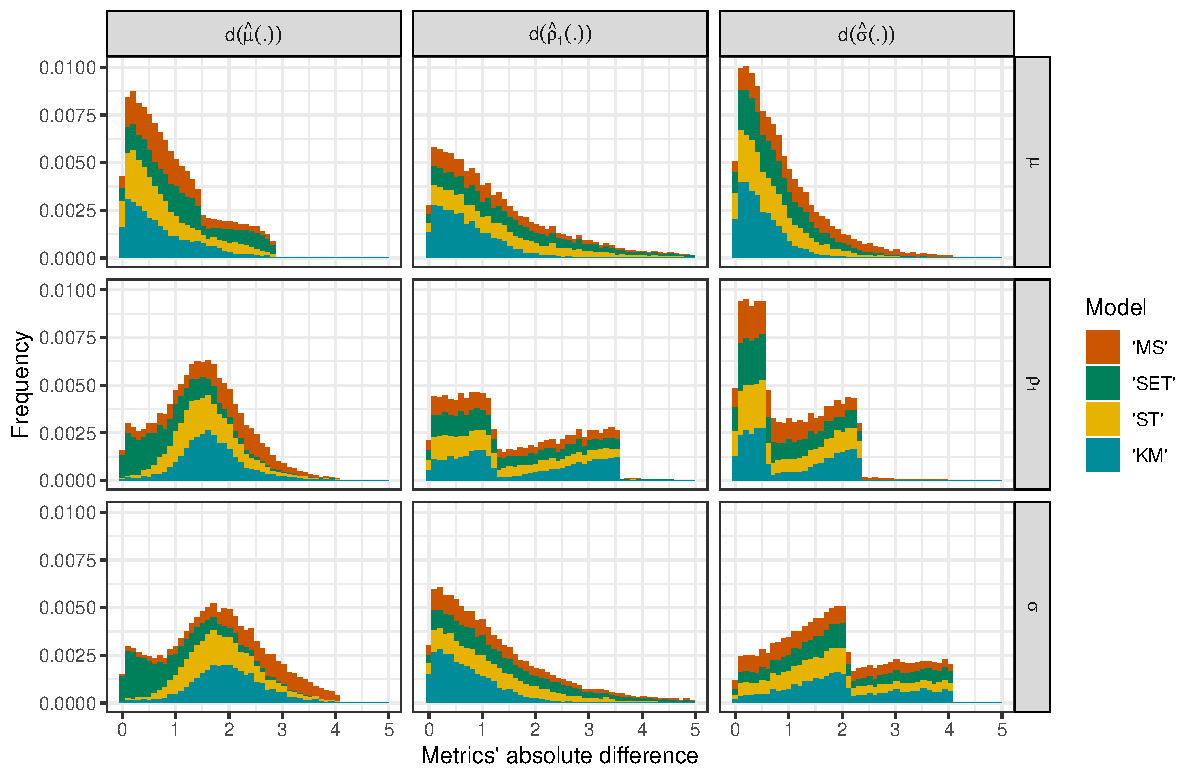
\includegraphics[width=\linewidth,height=0.75\textheight,keepaspectratio]{../../outputs/exploratory/metrics_diff.pdf}

}

\end{figure}%
\end{frame}

\section{Análise de performance}\label{anuxe1lise-de-performance}

\begin{frame}{Efeitos fixos dos modelos}
\phantomsection\label{efeitos-fixos-dos-modelos}
\begin{table}[!htbp]

\caption{\label{tbl-fe_strat}Efeitos fixos dos modelo}

\centering{

\vspace{-0.7cm}
\resizebox{\textwidth}{!}{%
    \begin{tabular}{@{\extracolsep{5pt}}lcccccc} 
\\[-1.8ex]\hline 
\hline \\[-1.8ex] 
\\[-1.8ex] & \multicolumn{6}{c}{RMSE} \\ 
\\[-1.8ex] & (1) & (2) & (3) & (4) & (5) & (6)\\ 
\hline \\[-1.8ex] 
 MS & 1.781$^{***}$ & 1.308$^{***}$ & 1.676$^{***}$ & 1.782$^{***}$ & 1.569$^{***}$ & 1.987$^{***}$ \\ 
  & (0.009) & (0.005) & (0.013) & (0.015) & (0.015) & (0.017) \\ 
  SET & 1.687$^{***}$ & 1.322$^{***}$ & 1.607$^{***}$ & 1.601$^{***}$ & 1.529$^{***}$ & 1.932$^{***}$ \\ 
  & (0.009) & (0.005) & (0.013) & (0.015) & (0.015) & (0.017) \\ 
  ST & 1.632$^{***}$ & 1.313$^{***}$ & 1.553$^{***}$ & 1.391$^{***}$ & 1.611$^{***}$ & 1.884$^{***}$ \\ 
  & (0.009) & (0.005) & (0.013) & (0.016) & (0.015) & (0.018) \\ 
  KM & 1.308$^{***}$ & 1.132$^{***}$ & 1.254$^{***}$ & 1.182$^{***}$ & 1.180$^{***}$ & 1.562$^{***}$ \\ 
  & (0.009) & (0.005) & (0.013) & (0.015) & (0.015) & (0.017) \\ 
  RF & 1.588$^{***}$ & 1.214$^{***}$ & 1.578$^{***}$ & 1.320$^{***}$ & 1.508$^{***}$ & 1.910$^{***}$ \\ 
  & (0.009) & (0.005) & (0.013) & (0.016) & (0.015) & (0.017) \\ 
  Strat. & none & asym. RGP & small RN & $\mu$ RN & $\rho_1$ RN & $\sigma$ RN \\
 \hline \\[-1.8ex] 
Observations & 99,944 & 44,491 & 50,172 & 32,357 & 33,925 & 33,662 \\ 
R$^{2}$ & 0.603 & 0.879 & 0.591 & 0.589 & 0.595 & 0.639 \\ 
Adjusted R$^{2}$ & 0.603 & 0.879 & 0.591 & 0.589 & 0.595 & 0.639 \\ 
Residual Std. Error & 1.302 & 0.467 & 1.280 & 1.229 & 1.224 & 1.398 \\ 
\hline 
\hline \\[-1.8ex] 
\textit{Note:}  & \multicolumn{6}{r}{$^{*}$p$<$0.1; $^{**}$p$<$0.05; $^{***}$p$<$0.01} \\ 
\end{tabular} 
%
}

}

\end{table}%
\end{frame}

\begin{frame}{Má-especificação e desempenho}
\phantomsection\label{muxe1-especificauxe7uxe3o-e-desempenho}
Má especificação da família do RGP diminui o desempenho:

\begin{itemize}
\tightlist
\item
  Efeito base de \(0.515\) (\(0.013\)).
\item
  MS tem efeito \(\approx 1.3\) vezes maior que SET e ST
\item
  Quando o RGP é sem-RS, o efeito é de \(3.531\) (\(0.014\)).
\item
  RN de \(\sigma\) tem efeito \(\approx 1.9\) vezes maior do que de
  \(\mu\) ou \(\rho\).
\item
  Mudança grande tem efeito \(\approx 1.4\) vezes maior que uma pequena.
\item
  Nenhum par modelo-RGP tem efeito significativamente diferente de
  outro, fora com o RGP sem-RS
\end{itemize}
\end{frame}

\begin{frame}{Modelos e características dos regimes}
\phantomsection\label{modelos-e-caracteruxedsticas-dos-regimes}
\begin{table}[!htbp]

\caption{\label{tbl-mis_metrics_sim}Modelos e `perfis' de métricas
condicionais veradeiras}

\centering{

\vspace{-0.5cm}
\resizebox{\textwidth}{!}{%
    \begin{table}[t]
\fontsize{12.0pt}{14.0pt}\selectfont
\begin{tabular*}{\linewidth}{@{\extracolsep{\fill}}l|rrr}
\toprule
RGP \(\diagdown\) Model & SET & ST & MS \\ 
\midrule\addlinespace[2.5pt]
SET & -0.054 (0.09) & -0.001 (0.068) & -0.009 (0.084) \\ 
ST & 1.482 (0.09)*** & -0.052 (0.068) & 0.157 (0.084)* \\ 
MS & 0.002 (0.091) & 0 (0.068) & -0.013 (0.084) \\ 
\bottomrule
\end{tabular*}
\begin{minipage}{\linewidth}
\vspace{.05em}
\emph{Note:}  \(^{*}\)p\$\textless{}\$0.1; \(^{**}\)p\$\textless{}\$0.05; \(^{***}\)p\$\textless{}\$0.01\\
\end{minipage}
\end{table}

%
}

}

\end{table}%

\emph{Porém:} com as métricas estimadas, os resultados mudam, e variam
entre RNs.
\end{frame}

\begin{frame}{Identificação e desempenho}
\phantomsection\label{identificauxe7uxe3o-e-desempenho}
\begin{table}[!htbp]

\caption{\label{tbl-match_r2}RMSE e identificação do fit e \(r\)}

\centering{

\vspace{-0.4cm}
\resizebox{0.8\textwidth}{!}{%
    \begin{tabular}{@{\extracolsep{5pt}}lcc} 
\\[-1.8ex]\hline 
\hline \\[-1.8ex] 
\\[-1.8ex] & \multicolumn{2}{c}{RMSE} \\ 
\\[-1.8ex] & $x = R^2$ & $x = BME(r)$\\ 
\hline \\[-1.8ex] 
  $x ~ \cdot$ No RS & 0.749$^{***}$ (0.009) & $-$0.914$^{***}$ (0.012) \\ 
  $x ~ \cdot$ MS & 0.746$^{***}$ (0.009) &    0.497$^{***}$ (0.021)     \\ 
  $x ~ \cdot$ SET & 0.851$^{***}$ (0.010) &   0.329$^{***}$ (0.018)     \\ 
  $x ~ \cdot$ ST & 0.849$^{***}$ (0.013) &    0.347$^{***}$ (0.012)     \\ 
  $x ~ \cdot$ KM & 0.467$^{***}$ (0.009) &    $-$0.310$^{***}$ (0.016)  \\ 
  $x ~ \cdot$ RF & 1.482$^{***}$ (0.011) &      \\ 
 \hline \\[-1.8ex] 
Observations & 120,850 & 100,840 \\ 
R$^{2}$ & 0.288 & 0.072 \\ 
Residual Std. Error & 1.786 & 2.039 \\ 
F Statistic p-value & <0.001 & <0.001 \\ 
\hline 
\hline \\[-1.8ex] 
\textit{Note:}  & \multicolumn{2}{r}{$^{*}$p$<$0.1; $^{**}$p$<$0.05; $^{***}$p$<$0.01} \\ 
\end{tabular} 
%
}

}

\end{table}%
\end{frame}

\begin{frame}{Identificação e desempenho}
\phantomsection\label{identificauxe7uxe3o-e-desempenho-1}
\begin{table}[!htbp]

\caption{\label{tbl-match_metrics}RMSE e identificação das métricas
condicionais}

\centering{

\vspace{-0.4cm}
\resizebox{\textwidth}{!}{%
    \begin{tabular}{@{\extracolsep{\fill}}l|rrr}
\toprule
 & \multicolumn{3}{c}{{RGP}} \\ 
\cmidrule(lr){2-4}
Model & SET & ST & MS \\ 
\midrule\addlinespace[2.5pt]
SET & 1.107*** (0.01) & 0.332*** (0.006) & 1.955*** (0.041) \\ 
ST & 0.234*** (0.004) & 0.976*** (0.041) & 1.884*** (0.042) \\ 
MS & 0.445*** (0.005) & 2.322*** (0.034) & 2.113*** (0.018) \\ 
\bottomrule
\end{tabular}
\begin{minipage}{\linewidth}\centering
\vspace{.05em}
\emph{Note:}  \(^{*}\)p\textless{}0.1; \(^{**}\)p\textless{}0.05; \(^{***}\)p\textless{}0.01\\
\end{minipage}
%
}

}

\end{table}%
\end{frame}

\begin{frame}{Má-especificação do número de regimes}
\phantomsection\label{muxe1-especificauxe7uxe3o-do-nuxfamero-de-regimes}
\begin{table}[!htbp]

\caption{\label{tbl-regimes}Má especificação do número de regimes}

\centering{

\vspace{-0.3cm}
\resizebox{0.8\textwidth}{!}{%
    \begin{tabular}{@{\extracolsep{5pt}}lccc} 
\\[-1.8ex]\hline 
\hline \\[-1.8ex] 
\\[-1.8ex] & \multicolumn{3}{c}{RMSE} \\ 
\\[-1.8ex] & (1) & (2) & (3)\\ 
\hline \\[-1.8ex] 
 $\hat{S} < S$ & $-$0.809$^{***}$ (0.017) &  & $-$0.494$^{***}$ (0.023) \\ 
  $\hat{S} > S$ & 0.714$^{***}$ (0.020) & 1.981$^{***}$ (0.028) &  \\ 
  $\hat{S} > S$ : $d(\hat{\mu}(.))$ &  & $-$1.927$^{***}$ (0.029) &  \\ 
  $\hat{S} > S$ : $d(\hat{\rho}_1(.))$ &  & $-$2.166$^{***}$ (0.096) &  \\ 
  $\hat{S} > S$ : $d(\hat{\sigma}(.))$ &  & $-$2.727$^{***}$ (0.050) &  \\ 
  $\hat{S} < S$ : $d(\hat{\mu}(.))$ &  &  & 0.301$^{***}$ (0.032) \\ 
  $\hat{S} < S$ : $d(\hat{\rho}_1(.))$ &  &  & 0.426$^{***}$ (0.111) \\ 
  $\hat{S} < S$ : $d(\hat{\sigma}(.))$ &  &  & 0.517$^{***}$ (0.054) \\ 
  Constant & 1.479$^{***}$ (0.013) & 1.183$^{***}$ (0.013) & 1.580$^{***}$ (0.017) \\ 
Strat. & none & none & no KM \\
 \hline \\[-1.8ex] 
Observations & 81,970 & 81,970 & 61,128 \\ 
R$^{2}$ & 0.498 & 0.519 & 0.537 \\ 
Residual Std. Error & 0.938 & 0.918 & 1.005 \\ 
F Statistic p-value & <0.001 & <0.001 & <0.001 \\ 
\hline 
\hline \\[-1.8ex] 
\textit{Note:}  & \multicolumn{3}{r}{$^{*}$p$<$0.1; $^{**}$p$<$0.05; $^{***}$p$<$0.01} \\ 
\end{tabular}
%
}

}

\end{table}%
\end{frame}

\section{Conclusão}\label{conclusuxe3o}

\begin{frame}{Conclusão}
\phantomsection\label{conclusuxe3o-1}
\begin{itemize}
\item
  Estudei os processos e modelos de RS, através das características das
  distribuições de seus regimes.
\item
  Defini uma estrutura teórica e de simulações de Monte Carlo, geral e
  expansível, mas foquei em objetos e exercícios específicos.
\end{itemize}

\pause

Resultados gerais:

\begin{itemize}
\tightlist
\item
  RGPs e RNs interagem significativamente, e as métricas condicionais
  recuperam algumas relações.
\item
  Modelos erram as métricas condicionais, a depender do modelo e RN;
  previsões ruins sob \(r\) impreciso.
\item
  Subestimar \(S\) é menos danoso com regimes similares, e superestimar
  \(S\) é menos danoso com regimes diferentes.
\end{itemize}
\end{frame}

\begin{frame}{Conclusão}
\phantomsection\label{conclusuxe3o-2}
Resultados dos modelos:

\begin{itemize}
\tightlist
\item
  K-means é um bom aproximador: melhor desempenho, consistente em
  diferentes DGPs, e boas previsões mesmo com \(r\) imprecisos.
\item
  Modelos de \emph{threshold} são similares, `gostam' de mudanças na
  média.
\item
  ST captura mudanças pequenas, é sensível às séries sem-RS, a mudanças
  em \(\rho\), e errar a volatilidade condicional.
\item
  MS lida com regimes assimétricos, sofre com má-especificações do RGP e
  errar métricas condicionais.
\end{itemize}

\pause

\textbf{Resultados apresentam fatos úteis para entender os processos e
modelos. A análise de modelos \(\times\) métricas tem potencial para
recomendações práticas.}
\end{frame}

\begin{frame}{Limitações}
\phantomsection\label{limitauxe7uxf5es}
\textbf{Validade externa:} resultados condicionais na população de
processos geradores.

Melhoria: adicionar MS-ST, MS+T, outras distribuições para MS, e
transformações da variável de \emph{threshold}.

\textbf{Conjunto de métricas:} insuficiente para descrever interações
entre todos RGPs e RNs; de difícil estimação pelos modelos.

Melhoria: mais métricas (ex.: outros momentos), mais medidas de
dispersão, e versões ponderadas das métricas.
\end{frame}

\begin{frame}
\begin{center}
\Huge Obrigado!
\end{center}
\end{frame}




\end{document}
